\documentclass[a4paper]{article}

\usepackage[T1]{fontenc}
\usepackage[utf8x]{inputenc}

\usepackage[a4paper]{geometry}
\geometry{verbose,tmargin=3cm,bmargin=3cm,lmargin=2cm,rmargin=2cm,headheight=2cm,headsep=1cm,footskip=2cm}


\usepackage{fancyhdr}
\usepackage{enumerate}
\usepackage{adjustbox}
\pagestyle{fancy}
\setlength{\parskip}{\medskipamount}
\setlength{\parindent}{0pt}
\usepackage{graphicx}
\usepackage{listings}

\makeatletter

\usepackage{subcaption}
\usepackage{varwidth}
\usepackage{float} 
\usepackage{color}
\usepackage{lastpage}
\usepackage{indentfirst}

\lhead[lh-even]{Edgar Vedvik\\edgarmv}
\chead[ch-even]{TDT4230 Graphics and Visualization\\Assignment 1}
\rhead[rh-even]{\today}

\lfoot[lf-even]{}
\cfoot[cf-even]{Page \thepage{} of \pageref{LastPage}}
\rfoot[rf-even]{}

\date{}
\makeatother
\usepackage[english]{babel}

\begin{document}
\thispagestyle{fancy}

\section{Texturing}
\subsubsection*{Question 4}

    The textured square can be seen in Figure \ref{fig:textured_diamond}. The
    minification and magnification sampling filters are both \emph{GL\_LINEAR}.
    
    \begin{figure}[H]
        
\includegraphics[width=\linewidth]{textured_diamond}
        \caption{A square textured with the diamond.png texture.}
        \label{fig:textured_diamond}
    \end{figure}

\subsubsection*{Question 5}
    Set the minification and magnification filters to be \emph{GL\_NEAREST}.
    Mipmapping should still be used to remove aliasing. So
    \emph{GL\_NEAREST\_MIPMAP\_NEAREST} could be used to achieve this. 

\subsubsection*{Question 6}
    Mipmaps are a sequence of images that each have a progressively lower
    resolution. This is done for two reasons: better performance and reduction
    of aliasing. The performance gains is because textures further away can use
    a lower resolution texture. It also reduced aliasing because the textured
    sampled from has a lower resolution, meaning there are fewer pixels to be
    sampled from.

\subsubsection*{Question 8}

    The texture gets blurry. Mipmaps causes this because the texture is now
    small, so a low resolution texture is being sampled from. Linear filtering
    gives the weighted average of the closest pixels, but when there are so few
    pixels, they end up looking a little blurry.

    \begin{figure}[H]
        
\includegraphics[width=\linewidth]{small_texture}
        \caption{A small square textured with mipmaps}
        \label{fig:small_texture}
    \end{figure}

\subsubsection*{Question 9}
    Anisotropic filtering produces a better looking image than mipmaps and
    linear filtering because it reduces blur and provides a better view at
    obtuse angles. The trade-off, however, is that anisotropic filtering is
    computationally expensive.

\section{Lighting}
\subsubsection*{Question 10}
    The amount of light the diffuse component reflects depends on the normal of
    the surface. This means that the larger the angle between the light source
    and the surface normal the less light it will create.

\subsubsection*{Question 11}
    Global illumination is a technique that add more realistic lighting to 3D
    scenes by taking into account both direct and indirect illumination.
    This means that a surface is lighted up directly by a light source, but also
    by light rays that have bounced of other surfaces in the scene. This
    procedure is not (yet) suitable for real time rendering because of the
    amount of processing that is required. 

\subsubsection*{Question 15}

    \begin{figure}[H]
        \centering
        \hfill
        \begin{subfigure}{.32\linewidth}%
            
\includegraphics[width=\linewidth]{ambient}
            \caption{Only ambient lighting.}
        \end{subfigure}
        \begin{subfigure}{.32\linewidth}%
            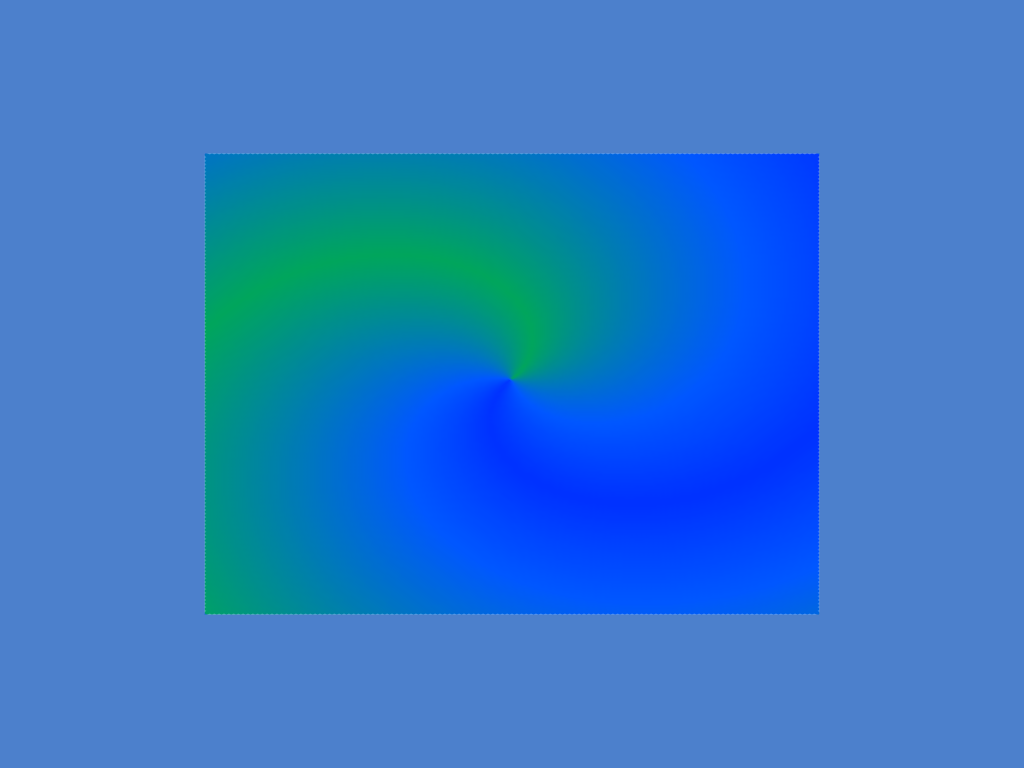
\includegraphics[width=\linewidth]{diffuse}
            \caption{Ambient and diffuse.}
        \end{subfigure}
        \begin{subfigure}{.32\linewidth}%
            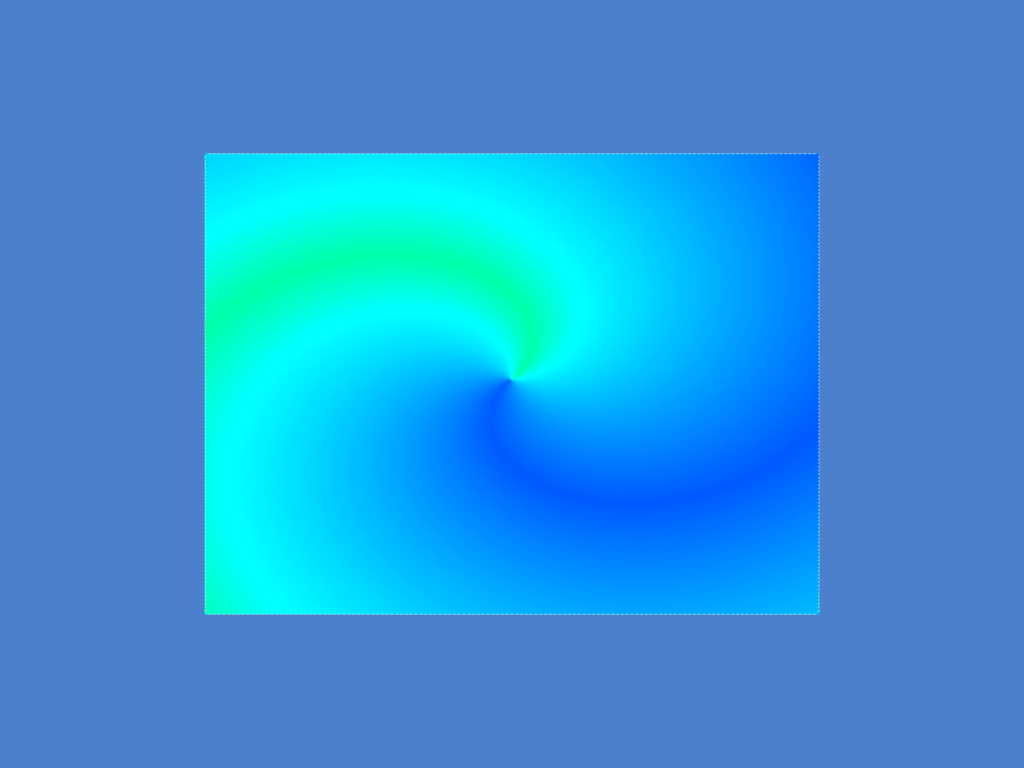
\includegraphics[width=\linewidth]{specular}
            \caption{Ambient, diffuse and specular.}
        \end{subfigure}
        \caption{Three screenshots from different points in time.}
        \label{fig:lighting}
    \end{figure}

\subsubsection*{Question 16}

    Gouraud shading will produce worse looking images when the vertex count for
    a model is low. Specular lighting will look very unnatural as it is
    calculated for vertices. So when there are few vertices the specular
    lighting will fade in and out as it moves from vertex to vertex, instead of
    providing a smooth transition like in Phong.

\end{document}
